\documentclass[11pt]{article}
\usepackage{deauthor}
\usepackage{times,graphicx,color,xspace}
\usepackage{listings}
\usepackage{hyperref}
\usepackage{subfig}
\newcommand{\mpv}[1]{\textcolor{blue}{mpv: #1}}
\newcommand{\rd}[1]{\textcolor{red}{rd: #1}}
\newcommand{\mlwfs}{ML workflows\xspace}
\newcommand{\mdb}{{\sc ModelDB}\xspace}
\newcommand{\mlwf}{ML workflow\xspace}
\newcommand{\wf}{workflow\xspace}
\newcommand{\wfs}{workflows\xspace}
\newcommand{\Dss}{Data scientists\xspace}
\newcommand{\Ds}{Data scientist\xspace}
\newcommand{\dss}{data scientists\xspace}
\newcommand{\ds}{data scientist\xspace}
\newcommand{\mldevs}{ML developers\xspace}
\newcommand{\mldev}{ML developer\xspace}
\newcommand{\IWE}{We\xspace}
\newcommand{\iwe}{we\xspace}


% \graphicspath{{figs/}}

\title{{\sc ModelDB}: Opportunities and Challenges in Managing Machine Learning Models}
\author{
  Manasi Vartak\\
  MIT CSAIL \\
  \texttt{mvartak@csail.mit.edu}
  \and
  Samuel Madden\\
  MIT CSAIL \\
  \texttt{madden@csail.mit.edu}
}

\begin{document}
\maketitle
\begin{abstract}
Machine learning applications have become ubiquitous in a variety of domains.
Powering each of these ML applications are one or more machine learning models that are used to make key decisions or compute key quantities.
The life-cycle of an ML model starts with data processing, going on to feature engineering, model experimentation, deployment, and maintenance.
We call the process of tracking a model across all phases of its life-cycle as {\bf model management}.
In this paper, we discuss the current need for model management and describe \mdb, the first open-source model management system developed at MIT.
We also discuss the changing landscape and growing challenges and opportunities in managing models. 
\end{abstract}
\section{Introduction}
\label{sec:model-management}

Machine learning (ML) has become ubiquitous in a variety of applications including voice assistants, self-driving cars, and recommendation systems.
Each ML-based application employs one or more machine learning models that are used to make key decisions or compute key quantities such as recognizing spoken words, detecting a pedestrian on the road, and identifying the best products for customers.
Models are to ML-based applications what databases are to stateful web-applications; they are crucial for the correct functioning of these applications.
Consequently, just as database management systems (or DBMSs) are used to manage state in applications, we find the need for systems to manage models in ML applications, i.e., {\it model management systems}.

% While a DBMS serves the purpose of managing data throughout its life-cycle (i.e., creation, querying, update, and delete); a model management system serves the purpose of storing and querying {\it metadata} about models throughout their life-cycle.

% We begin with a brief overview of a typical model life-cycle and use it to motivate the need for model management.
To understand the requirements of a model management system, we begin with a brief overview of the life-cycle of a machine learning model.
We divide the ML life-cycle into five phases, namely:
% \begin{enumerate}
%     \item {\em Data Preparation} - Obtaining the training and test data to develop a model;
%     \item {\em Feature Engineering} - Identifying or creating the appropriate descriptors from the input data (i.e., features) to be used by the model; 
%     \item {\em Model Training and Experimentation} - Experimenting with different models on the training and test data and choosing the best; 
%     \item {\em Deployment} - Deploying the chosen model in a live system; and
%     \item {\em Maintenance} - Monitoring the live model performance, updating the model as needed, and eventually retiring the model.
% \end{enumerate}
(1) {\em Data Preparation} - Obtaining the training and test data to develop a model; 
(2) {\em Feature Engineering} - Identifying or creating the appropriate descriptors from the input data (i.e., features) to be used by the model; 
(3) {\em Model Training and Experimentation} - Experimenting with different models on the training and test data and choosing the best; 
(4) {\em Deployment} - Deploying the chosen model in a live system; and
(5) {\em Maintenance} - Monitoring the live model performance, updating the model as needed, and eventually retiring the model.
While we describe these phases as occurring in a linear sequence, the empirical nature of building an ML model causes multiple phases to be revisited frequently.
We define a model management system as one that follows a model throughout the five phases of its life-cycle and captures relevant metadata at each step to enable model tracking, reproducibility, collaboration, and governance.
% Since developing a high quality machine learning model is heavily dependent on data and the task, many of these steps are iterative.
% \mpv{Key requirements for what}
% At every phase of the model life-cycle, certain pieces of metadata are essential for ensuring that the model performs well, can be reproduced

% the \mpv{key requirements} at that phase.
% For example, for Phases 1-2, the key requirement for a model in that phase is reproducibility, i.e., enough data about the data preparation and feature engineering must be tracked so that the said features can be re-created exactly.
% Similarly, for Phase 3, the key requirement, along with reproducibility, is experiment tracking so that a \dss can choose the best model.
% For Phases 4-5, the key requirements deal with making model-related data widely accessible and ensuring that key metrics for the models are collected regularly.

\newpage

% Model management, at this time, is a loosely defined term used to capture different operations one might wish to perform when building or operationalizing machine learning models.
% We define a model management system as one that follows a model (whether deployed or not) throughout these five phases of its life-cycle and captures relevant metadata at each step.
For instance, since the key requirement during the Experimentation phase is to enable the \dss to choose the best model, metadata captured in this phase includes items such as performance metrics for the model, hyperparameter values used during training, etc.
In contrast, for a model in the Deployment phase, metadata might include the version of the model, where it is deployed, and how to query it.
Although one can imagine a model management system that directly stores models and supports prediction serving operations, the heterogeneity in models, as well as their hardware and software requirements make such a solution sub-optimal.
Therefore, we take the view that model management systems are best suited to store {\it metadata} about models throughout their life-cycle.
Thus, {\bf we define a model management system as a system that tracks metadata about models through the five phases of their life-cycle}.

% As machine learning deployments are becoming ubiquitous, various systems have been
% developed in academia and in industry to manage the life-cycle of \mlwfs.
% To the best of our knowledge, \mdb is the first open-source system for model
% management.

Given the rapid proliferation of machine learning applications, systems have been proposed in academia as well as industry to address different aspects of the model management problem.
In this paper, we focus on \mdb, the first open-source system we developed at MIT for model management.
Other academic systems that seek to address similar problems include the ModelHub system~\cite{modelhub} (to explore deep learning architectures and efficiently store network weights), 
ProvDB~\cite{provdb} (to manage 
metadata collected via collaborative data science), Ground~\cite{hellerstein2017ground} (to provide a common
framework for tracking data origin and use via generic abstractions), and the work on model selection management systems by Kumar et. al.~\cite{msms}.

An example of a commercial model management system is the SAS Model Manager which tracks models built and deployed within the SAS platform~\cite{sas-model-manager}.
Today, most proprietary ML platforms such as the Michelangelo platform at Uber~\cite{michelangelo} and FBLearner at Facebook~\cite{fblearner} include a model management or model repository component.
Similarly, vast majority of data science teams end up re-building a model management system to suit their needs.
In~\cite{sculley2014high-interest-cc}, Sculley et. al. elegantly present the
challenges with building and productionizing ML at Google and highlight the need to manage ``pipeline jungles'' and model configurations.
% Two of the problems highlighted in~\cite{sculley2014high-interest-cc} are the 
% technical debt arising from ``pipeline jungles'' and large amount of configurations.
% \mdb takes first steps in addressing these problems by providing a central
% repository where pipelines (i.e., \wfs) and their configurations are stored in
% a standardized format.
% Different companies have since published the architecture of their proprietary
% ML platforms such as the Michelangelo platform at Uber~\cite{michelangelo} and FBLearner at Facebook~\cite{fblearner}.
% These architectures have a model repository as a centerpiece.
% Similarly, in~\cite{schibsted-versioning-pipelines} authors describe a 
% proprietary pipeline versioning system developed to track ML pipelines. 
% Unlike \mdb, this system performs versioning at the pipeline-stage granularity 
% and versions not only the operators used at each stage but also the intermediate
% datasets produced by each stage. 

Model management systems are also closely related to workflow and experiment management systems such as Kepler~\cite{kepler}, Taverna workbench~\cite{taverna},
Galaxy~\cite{galaxy}, VisTrails~\cite{bavoil2005vistrails, callahan2006vistrails, callahan2006workflows} as well as recently introduced workflow engines tailored for data processing such as Apache Airflow~\cite{airflow} and
Luigi~\cite{luigi}.
While workflow systems can address some of the model management needs during the first three phases of the model life-cycle, these systems require extensions for ML-specific abstractions.
% A hybrid approach is used by new \wf system such as Apache Airflow~\cite{airflow} and
% Luigi~\cite{luigi} where \wfs are defined in code but the steps must follow a uniform interface.
% For example, \wfs in Apache Airflow are DAGs of Tasks where a Task implements the
% common Operator interface.
% Every execution of the DAG creates a Run that is executed with the particular 
% task instances.
% Defining \wfs in code enables \mldevs to use their preferred ML or data processing
% libraries while still making it easy to track and run \wfs.


% A major drawback of VisTrails and most of the scientific workflow systems 
% described above is that they require scientists to use a system-specific \wf
% definition interface (GUI or otherwise) that is separate from their scientific
% development environment.
% This is, in fact, the solution also adopted by some commercial ML systems including
% Microsoft Azure ML~\cite{azure-ml} and the SeaHorse product from DeepSense~\cite{seahorse}.
% From our interviews with dozens of data scientists, however, we learned that 
% \dss found the use of a standalone workflow management systems (particularly 
% GUI-based) extremely restrictive.
% \Dss want the freedom to write workflows in their ML environment of 
% choice and the ability to use new ML techniques without waiting
% for the \wf management system to reflect these updates.
% Moreover, we found that \dss were unwilling to switch to new tools for one piece 
% of functionality (however key the functionality may be).
% Thus we found that while a standalone workflow specification system would be 
% much easier to build, it would have immense difficulty getting adoption with \mldevs. 
% As a result, a significant part of the effort in designing and implementing \mdb
% was directed towards passively collecting \mlwfs without requiring \dss to 
% change their modeling processes.

The rest of the paper is organized as follows.
In Section~\ref{sec:motivation}, we describe the motivation behind model management systems; in Section~\ref{sec:challenges}, we describe the challenges faced in building model management systems; and in Section~\ref{sec:modeldb}, we describe the \mdb system developed at MIT.
We conclude the paper in Section~\ref{sec:future} with a discussion of how we see model management evolving in the future.

% A key part of this paper seeks to define what model management means to data science and machine learning practitioners and how that translates to a need for a model management system.
% Models are to ML-based applications what databases are to web-applications \mpv{??}.
% They are key for the correct functioning of these applications.
% Consequently, just like we have database management systems (or DBMSs), we find the need for systems that manage models.
% While a DBMS serves the purpose of storing, querying, and updating data; a model management system serves the purpose of storing metadata about models, optionally the models, enable querying of the metadata and models.
% Unlike database systems, model management systems are more concerned with storing model metadata as opposed to the models themselves.
% The reason is that machine learning models are often extremely diverse and do not follow a fixed schema.
% In this paper, we focus on \mdb, a system we developed at MIT to address the problem of model management while building an ML model.
% We provide a perspective on the challenges in model management and how we see the need for model management evolve in the future.
\section{Why Model Management?}
\label{sec:motivation}

To understand the need for model management, we studied modeling workflows across companies and research labs ranging from large internet companies to small start-ups building ML-based applications.
Across the different phases of the model life-cycle, the need for model management was apparent in three key areas: managing modeling experiments, enabling reproducibility, supporting sharing of models, and model governance.

The first and primary area where the need for model management is evident is during the Experimentation phase of the model life-cycle.
The empirical nature of ML model development means that \dss and \mldevs experiment with hundreds of models before identifying one that meets some acceptance criteria.
This is particularly true when \dss perform hyperparameter optimization on models.
Data about previously built models is necessary to inform the next set of models and experiments, and to identify the best model produced so far.
Consequently, tracking these experiments is of paramount importance.
The absence of an experiment tracking system leads to models and experiments being lost and valuable time and resources being spent in reproducing model results.
For example, one \mldev at a large tech company related how she had spent over a week merely re-running a modeling experiment another employee had previously conducted since the experimental setup and results were not recorded.

The second area that requires model management is enabling model reproducibility.
A key use case for reproducibility deals with the situation where the new version of a deployed model performs poorly compared to the previous one and must be reverted to the older version.
If the previous model version is not available, re-creating it requires precise information about what data was used, how it was processed, libraries and versions used, and details of how the model was trained (including random seeds).
A similar need becomes evident when a model has to be updated with new data or when a discrepancy is detected in an offline and live model.

The third area that requires model management is supporting model sharing.
As data science teams increase in size, multiple \dss want to collaborate on the same model or build on top of each others' work.
In such cases, the lack of a centralized repository of models along with the right access control patterns hampers sharing of information about models and experiments.
Finally, for software developers who wish to use existing ML models, the absence of a central repository makes it challenging to discover and integrate models into products and business processes.
% Similarly, when data science teams want to collaborate on a particular model or build on top of each other's work (e.g., use the results of one model as input to another), 
    
The last area where we find a growing need for model management relates to model governance. 
% In non-regulated industries, model governance often translates only to business insight into models used in a product or business.
For many regulated industries, (e.g., banking and healthcare), government regulations require that any model used to make automated decisions be documented and available for audit. 
Furthermore, government legislation now being implemented (e.g., the GDPR regulations in the European Union~\cite{gdpr}) requires that companies be able to explain any decisions made without human intervention.
These trends highlight the need for a centralized system that manages and explains models.
% All of these requirements make it essential to provide a centralized repository
% making it essential to record all models and explain their predictions.

\section{Challenges in Model Management}
\label{sec:challenges}

As defined above, model management covers the entire life-cycle of models starting with Data Processing, Feature Engineering, Experimentation, Deployment, and Maintenance.
The hallmark of machine learning model development is the heterogenity in environments and frameworks used at every phase of the ML life-cycle.
As a result, the primary challenge for model management is to consistently capture metadata across many environments at each phase of the modeling life-cycle.
We illustrate this challenge with a few examples.
% Across all the above stages, {\it diversity} and {\it heterogeneity} in ML environments and frameworks are the key challenges in consistently capturing metadata across the modeling lifecycle.

During the Data Processing or Feature Engineering phases, our goal is to track the
transformations applied to data so that they may be accurately reproduced later.
% features that are created and used in a model.
Since these tasks may be done in very different languages and data processing environments (e.g., Spark, Teradata, HBase), we must ensure that data transformations can be accurately recorded across a wide range of data processing environments.
Moreover, even within a single environment, we must ensure high coverage for all the ways in which a specific data transformation may be applied --- a significant challenge unless this functionality has been built into the system from the ground-up.

Similarly, during the Experimentation phase, there is a large diversity in machine learning frameworks and libraries in different programming languages that a \ds may use (e.g., scikit-learn, Tensorflow, PyTorch in Python; ML libraries in R; H2O framework in Java).
Each library has a unique way of defining models (e.g., graphs in Tensorflow vs. plain objects in scikit-learn) and their associated attributes.
Consequently, one representation is often inadequate to capture models built across all frameworks.
This diversity in machine learning frameworks during Experimentation also translates to diversity in deployment methods during the Deployment phase.
For example, while TF-serving is a popular means to serve Tensorflow models, a Flask-based deployment method is most popular for scikit-learn models.
% Consistently capturing relevant deployment properties for all the deployment methods is challenging during the Deployment phase.
% This diversity produces similar model management challenges during the Deployment phase.

Lastly, once a model is deployed, i.e. during the Maintenance phase, while some properties are common to all models (e.g., latency of predictions, number of requests), many properties are application dependent (e.g., accuracy of model for new users on an e-commerce site) and might require input from disparate systems outside of the ML environment (e.g., prediction storage or logging systems).
Thus we see that addressing the heterogeneity at every phase of the modeling life-cycle is the key challenge for model management.
% As a result, metadata collection during Maintenance also requires the application to be extensible.

% Given this heterogeneity in each phase of the model life-cycle, developing common abstractions and methods for tracking metadata across diverse environments and frameworks is the key challenge for model management.

While the above challenges arise from the diversity of environments for ML, two overarching requirements emerge from the data scientists' perspective as well.
First, \dss want a model management solution that minimizes developer intervention and requires minimal changes to the current developer workflow.
For example, many \dss are resistant to choosing a new ML environment or significantly changing their modeling workflow to account for model management.
And second, \dss want a vendor and framework-neutral model management system so that they are not tied into one particular provider or framework and can choose the best solutions for the particular modeling task.

To summarize, in order to build a model management system, we must address the problem of supporting a variety of ML environments, imposing common abstractions across diverse environments, and capturing sufficient metadata while requiring minimal changes from \dss.
In the next section, we describe \mdb, an open-source model management system developed at MIT that takes the first steps in tackling the challenges identified above and focuses particularly on the Experimentation phase of the model life-cycle.

\section{\mdb}
\label{sec:modeldb}

\begin{figure}[tb] 
\centerline{
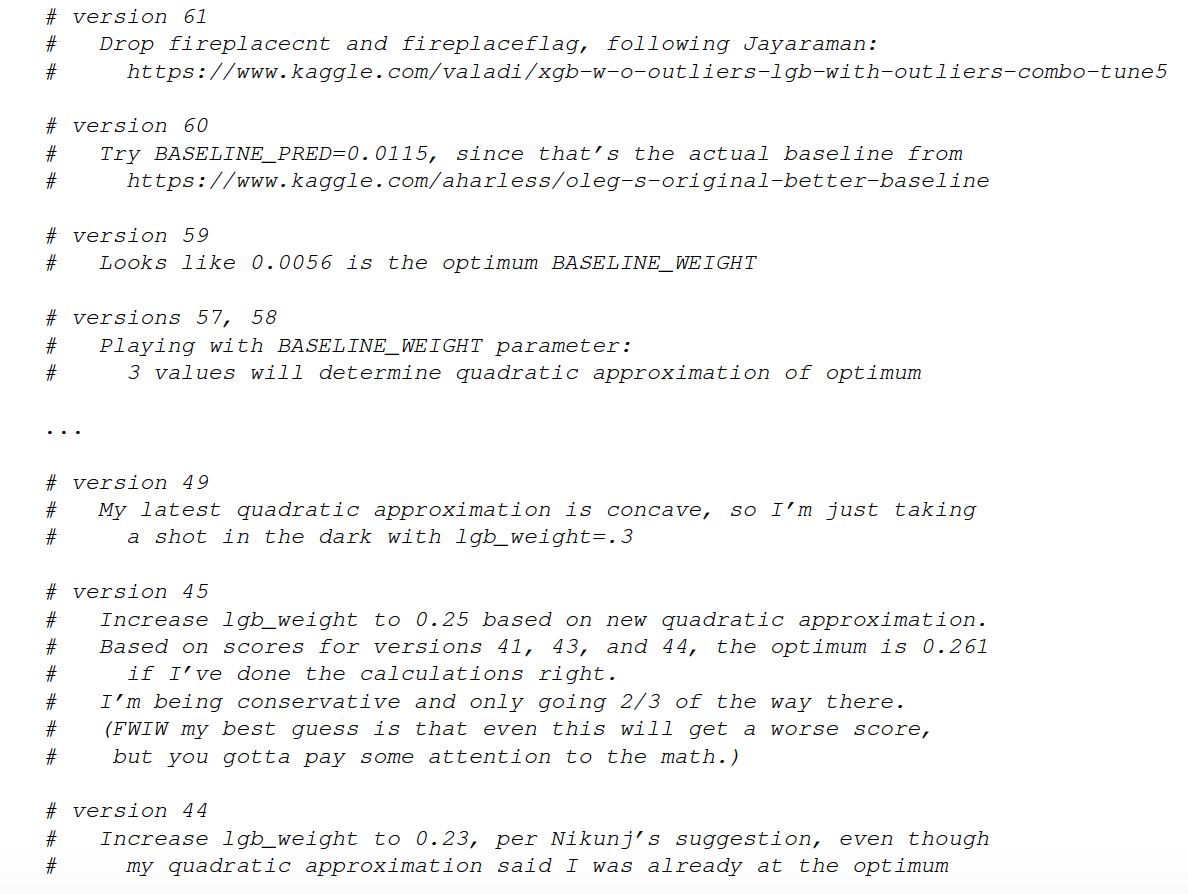
\includegraphics[trim=0mm 0mm 0mm 0mm,
width=0.85\textwidth,clip=true]{listing}}
\caption{Model Versioning comments by Kaggle competitor}
\label{lst:versioning_2}
\end{figure}

Building an ML model for real-world applications is an iterative process. 
\Dss and \mldevs experiment with tens to hundreds of models before identifying 
one that meets some acceptance criteria on model performance.
 % (e.g., mean squared error of predictions should be $<$0.05).
For example, top competitors in the Kaggle competition to predict Zillow Home prices~\cite{zillow} made more than 250 submissions (and therefore built at least as many models), while those in the Toxic Comment classification competition~\cite{toxic-comments} made over 400 submissions.
As an example of actual experimentation performed during model building, Figure~\ref{lst:versioning_2} reproduces code comments by an expert Kaggle competitor (ranked in top 500) written in order to track models built for the Zillow Price Prediction Challenge.
As we can see from this listing, a \ds typically tests a large number of model versions before identifying the best one.
Moreover, although \dss (and data science teams) build many tens to hundreds of models
when developing an ML application, they currently have no way to keep track of all 
the models they have built.
Consequently, insights are lost, models cannot be reproduced or shared, and model governance becomes challenging.
% \lstset{basicstyle=\tiny}
% \begin{lstlisting}[basicstyle=\small\ttfamily,caption={Model versioning comments by a Kaggle competitor},label={lst:versioning_2},language=Python]
% # version 61
% #   Drop fireplacecnt and fireplaceflag, following Jayaraman:
% #     https://www.kaggle.com/valadi/xgb-w-o-outliers-lgb-with-outliers-combo-tune5

% # version 60
% #   Try BASELINE_PRED=0.0115, since that's the actual baseline from
% #     https://www.kaggle.com/aharless/oleg-s-original-better-baseline

% # version 59
% #   Looks like 0.0056 is the optimum BASELINE_WEIGHT

% # versions 57, 58
% #   Playing with BASELINE_WEIGHT parameter:
% #     3 values will determine quadratic approximation of optimum

% ...

% # version 49
% #   My latest quadratic approximation is concave, so I'm just taking
% #     a shot in the dark with lgb_weight=.3

% # version 45
% #   Increase lgb_weight to 0.25 based on new quadratic approximation.
% #   Based on scores for versions 41, 43, and 44, the optimum is 0.261
% #     if I've done the calculations right.
% #   I'm being conservative and only going 2/3 of the way there.
% #   (FWIW my best guess is that even this will get a worse score,
% #    but you gotta pay some attention to the math.)

% # version 44
% #   Increase lgb_weight to 0.23, per Nikunj's suggestion, even though
% #     my quadratic approximation said I was already at the optimum
% \end{lstlisting}

% # version 55
% #   OK, it doesn't get the same result, but I also get a different result
% #     if I fork the earlier version and run it again.
% #   So something weird is going on (maybe software upgrade??)
% #   I'm just going to submit this version and make it my new benchmark.

% # version 53
% #   Re-parameterize ensemble (should get same result).

% # version 51
% #   Quadratic approximation based on last 3 submissions gives 0.3533
% #     as optimal lgb_weight.  To be slightly conservative,
% #     I'm rounding down to 0.35

% # version 50
% #   Quadratic approximation based on last 3 submissions gives 0.3073 
% #     as optimal lgb_weight

To address these problems, we developed a system at MIT called \mdb~\cite{modeldb-hilda}. 
\mdb is the first open-source machine learning model management system and currently focuses on tracking models during the Experimentation phase.
\mdb automatically tracks models as they are built, records 
provenance information for each step in the pipeline used to generate the model, stores this 
data in a standard format, and makes it available for querying via an API and a visual interface.
% In the following sections, we describe the architecture of \mdb, how data may be logged into the system and different ways of querying the data.
% We finish with a brief discussion of current work on extending \mdb.

% To address the problem of \mlwf management, 
% we propose a novel system called \mdb.
% \mdb is a centralized repository of models that tracks what models were built, how they were built (including pre-processing steps), and how they performed.
% To provide this functionality, 

% in their native environment (e.g., spark.ml or scikit-learn), indexes them intelligently, and allows flexible exploration of models via an API as well as a visual interface. 

\subsection{Architecture}

Figure \ref{fig:mdb_arch} shows the high-level architecture of our system. 
\mdb consists of three key components: client libraries for different machine learning environments, a backend that stores
model data, and a web-based visualization interface. 
Client libraries are responsible for automatically extracting models and pipelines from code
and passing them to the \mdb backend. 
The \mdb backend exposes a thrift\footnote{https://thrift.apache.org/} 
interface to allow clients in different 
languages to communicate with the \mdb backend.
\mdb client libraries are currently available for scikit-learn and spark.ml, along with a Light Python API that can be used in any Python-based machine learning environment.
This means that \mldevs can continue to build models and perform 
experimentation in these environments while the native libraries
passively capture model metadata.
% \mdb stores models and pipelines as a sequence of actions (as opposed to states) and uses a branching model of history to track the changes in models over time~\cite{Derthick01enhancingdata}. \mpv{FIX}
%Together, these abstractions can provide a chronicle of the users' model building operations in a format that can be easily shared, queried and visualized. 
The backend can use a variety of storage systems to store the model metadata.
% For ease of implementation, we chose to store \mdb generated model data in a
% relational database whereas for model metadata that can have a flexible schema 
% (e.g., user-specified key-value pairs or Light API specifications), we chose to use a key-value store.
The third component of \mdb, the visual interface, provides an easy-to-navigate layer on top of the backend storage system that permits visual exploration and analyses of model metadata.

\begin{figure}[tb] 
\centerline{
\hbox{\resizebox{10cm}{!}{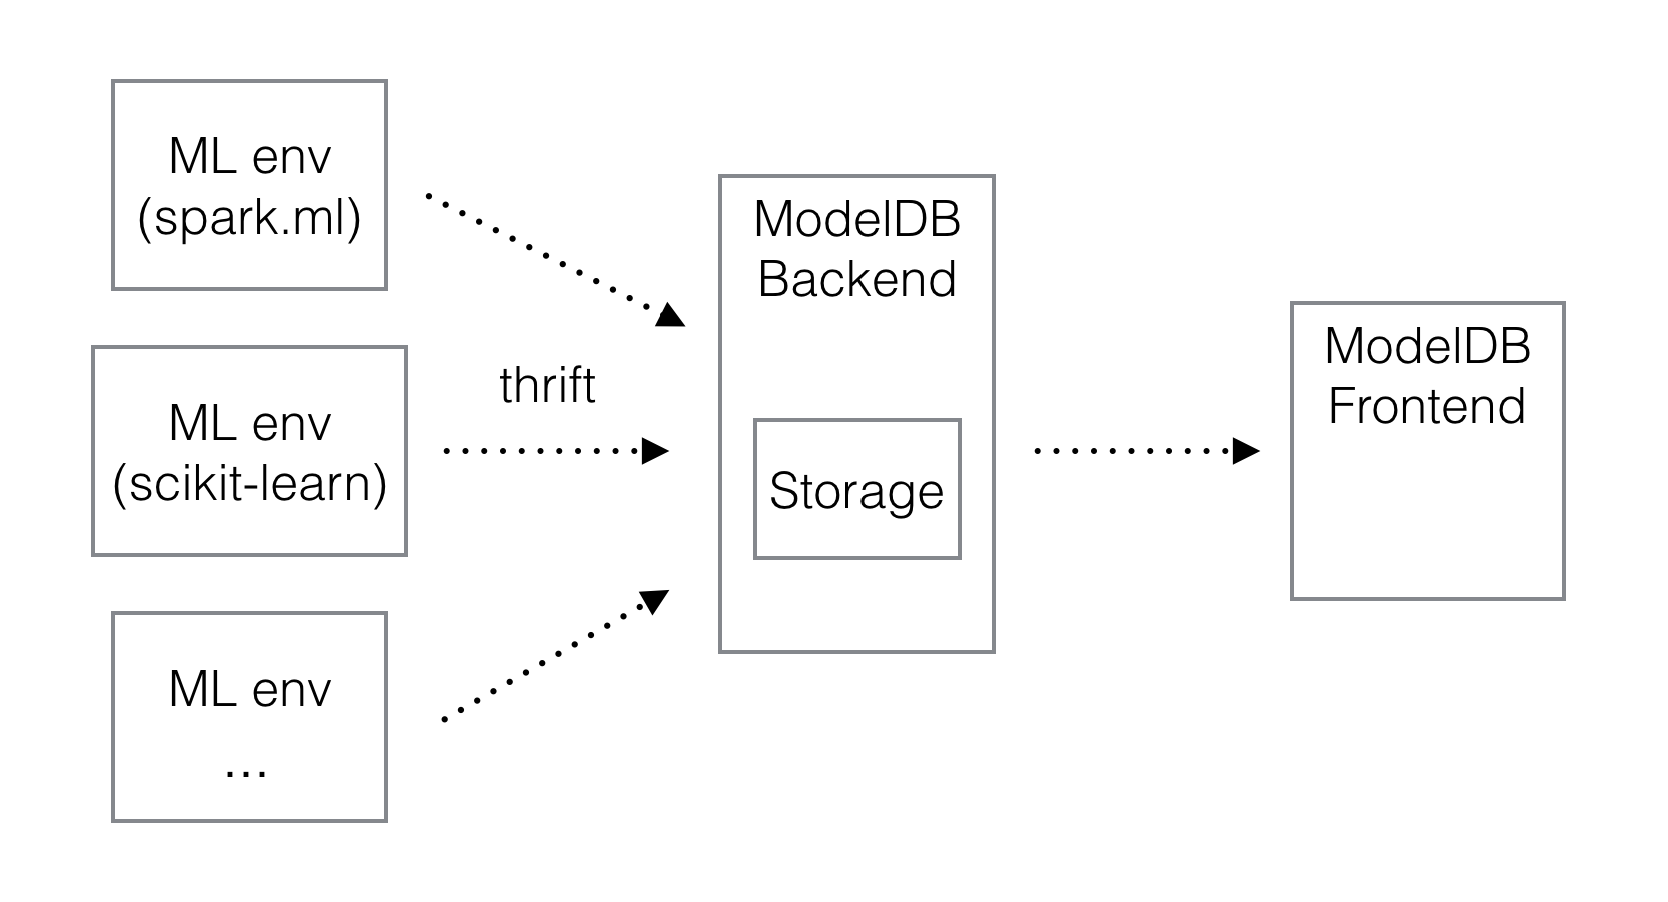
\includegraphics[trim=0mm 0mm 0mm 0mm,
clip=true]{mdb_arch.png}}}}
\caption{ModelDB Architecture}
\label{fig:mdb_arch}
\end{figure}
\subsection{Client Libraries}
Many existing workflow management programs (e.g. VisTrails~\cite{callahan2006vistrails}) require that the user create a workflow in advance, usually by means of a GUI. 
However, the \dss we interviewed overwhelmingly concurred that GUIs restricted their flexibility in defining modeling pipelines and iterating over them. 
Moreover, we found that \dss were resistant to significant changes in their modeling workflows.
Therefore, our primary design constraint while creating the \mdb client libraries was to minimize any changes the \ds would need to make both to code and the existing modeling process. To meet this constraint, we chose to make model logging accessible directly through code (as opposed to a GUI) and to build logging libraries for different ML environment. 
The spark.ml and scikit-learn libraries are architected such that \dss can use these environments for analysis exactly as they normally would and the library transparently and automatically logs the relevant data to the backend.
\subsection{Frontend}
\label{sec:mdb_frontend}

\mdb captures a large amount of metadata about models.
To support easy access to this data, \mdb provides a visual interface.
We provide three key views for exploring the data stored in \mdb.
A user starts with the projects summary page (Fig.~\ref{fig:project-summary}) 
that provides a high level overview of all the projects in the system.
The user can then click on a particular project to see the models for that project.
We present models via two key views.
The first view presents model summaries through two visualizations (Fig.~\ref{fig:mdb_model_timeline}): a summary visualization showing the evolution of model metrics over time as well as a custom visualization builder for model meta-analyses.
The second is a tabular view of models in a particular project (Fig.~\ref{fig:tabular-view}) along with interactions such as filtering, sorting, grouping, and search.
From any of the above interfaces, the \mldev can drill-down into a single model to visualize the model pipeline that was automatically inferred by the client library.
% (Fig.~\ref{fig:mdb_model_pipeline}) 

\begin{figure*}
  \centering
  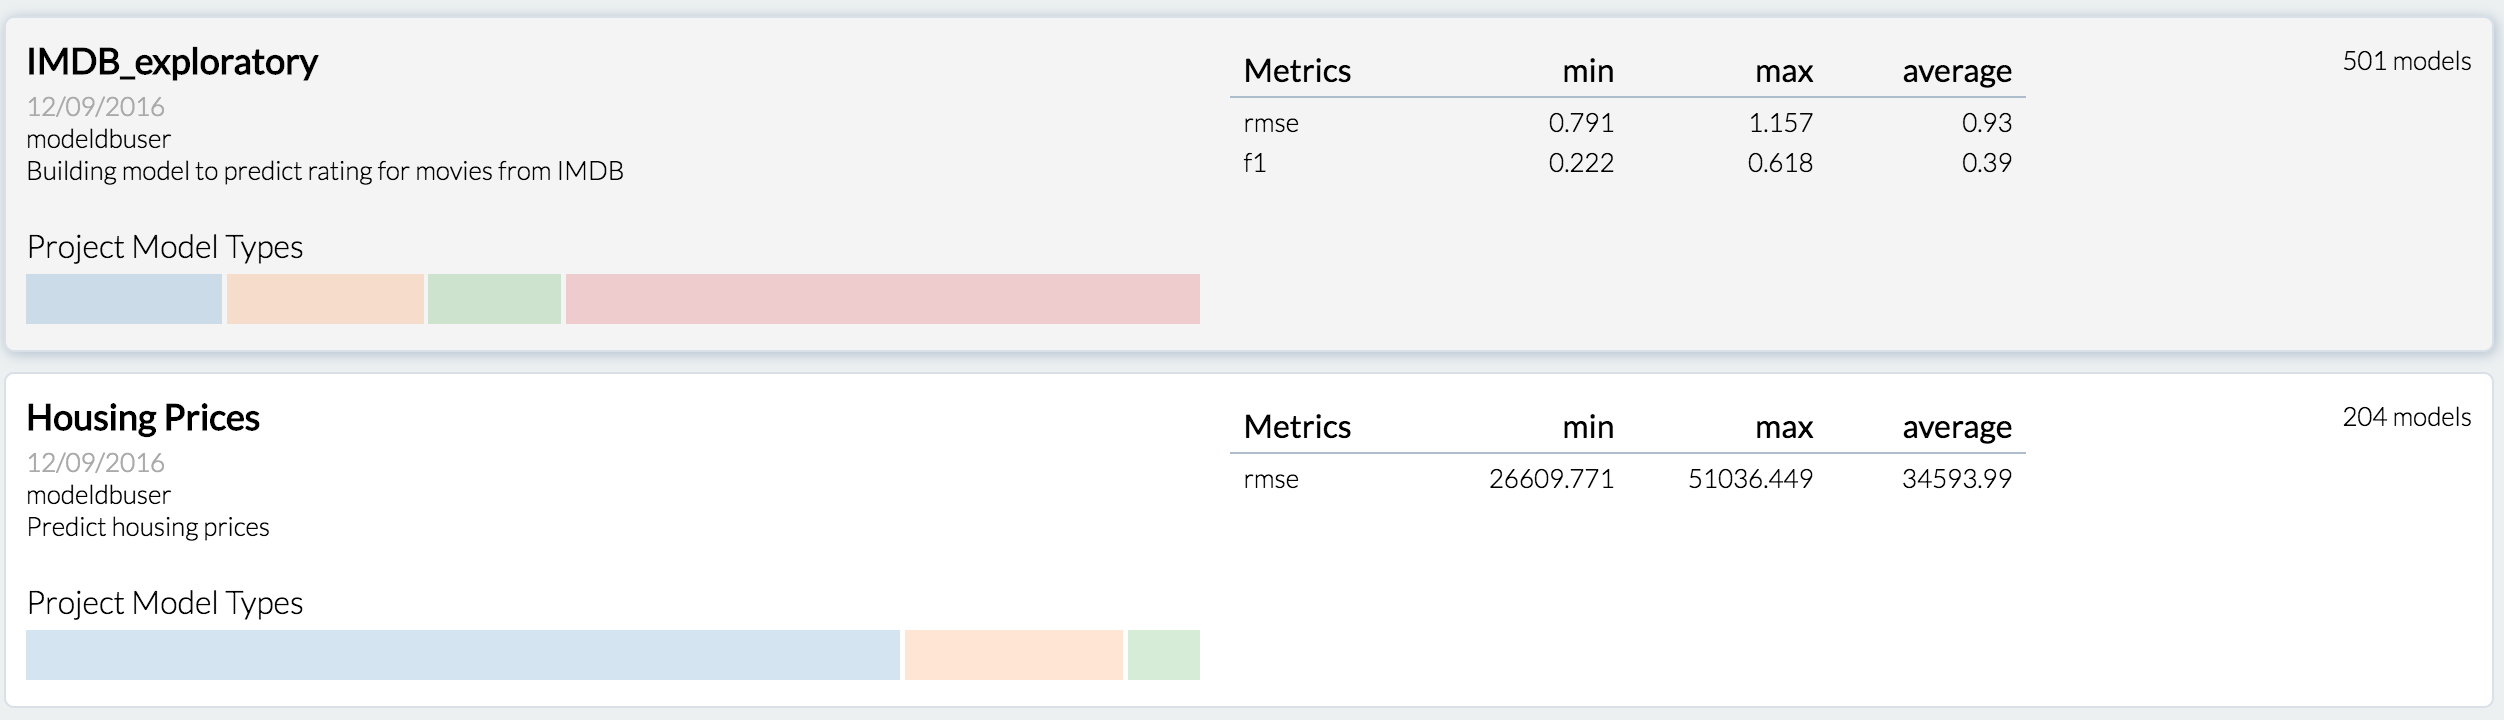
\includegraphics[trim=0mm 0mm 0mm 0mm,
  clip=true, width=\textwidth]{mdb_dashboard.png}
  \caption{\label{fig:project-summary} Projects Summary View}
\end{figure*}

% \begin{figure*}
% \centering
% \begin{subfig}
%   \centering
%   \includegraphics[width=0.48\textwidth]{figs/mdb_tabular.png}
% \end{subfig}%
% \begin{subfigure}
%   \centering
%   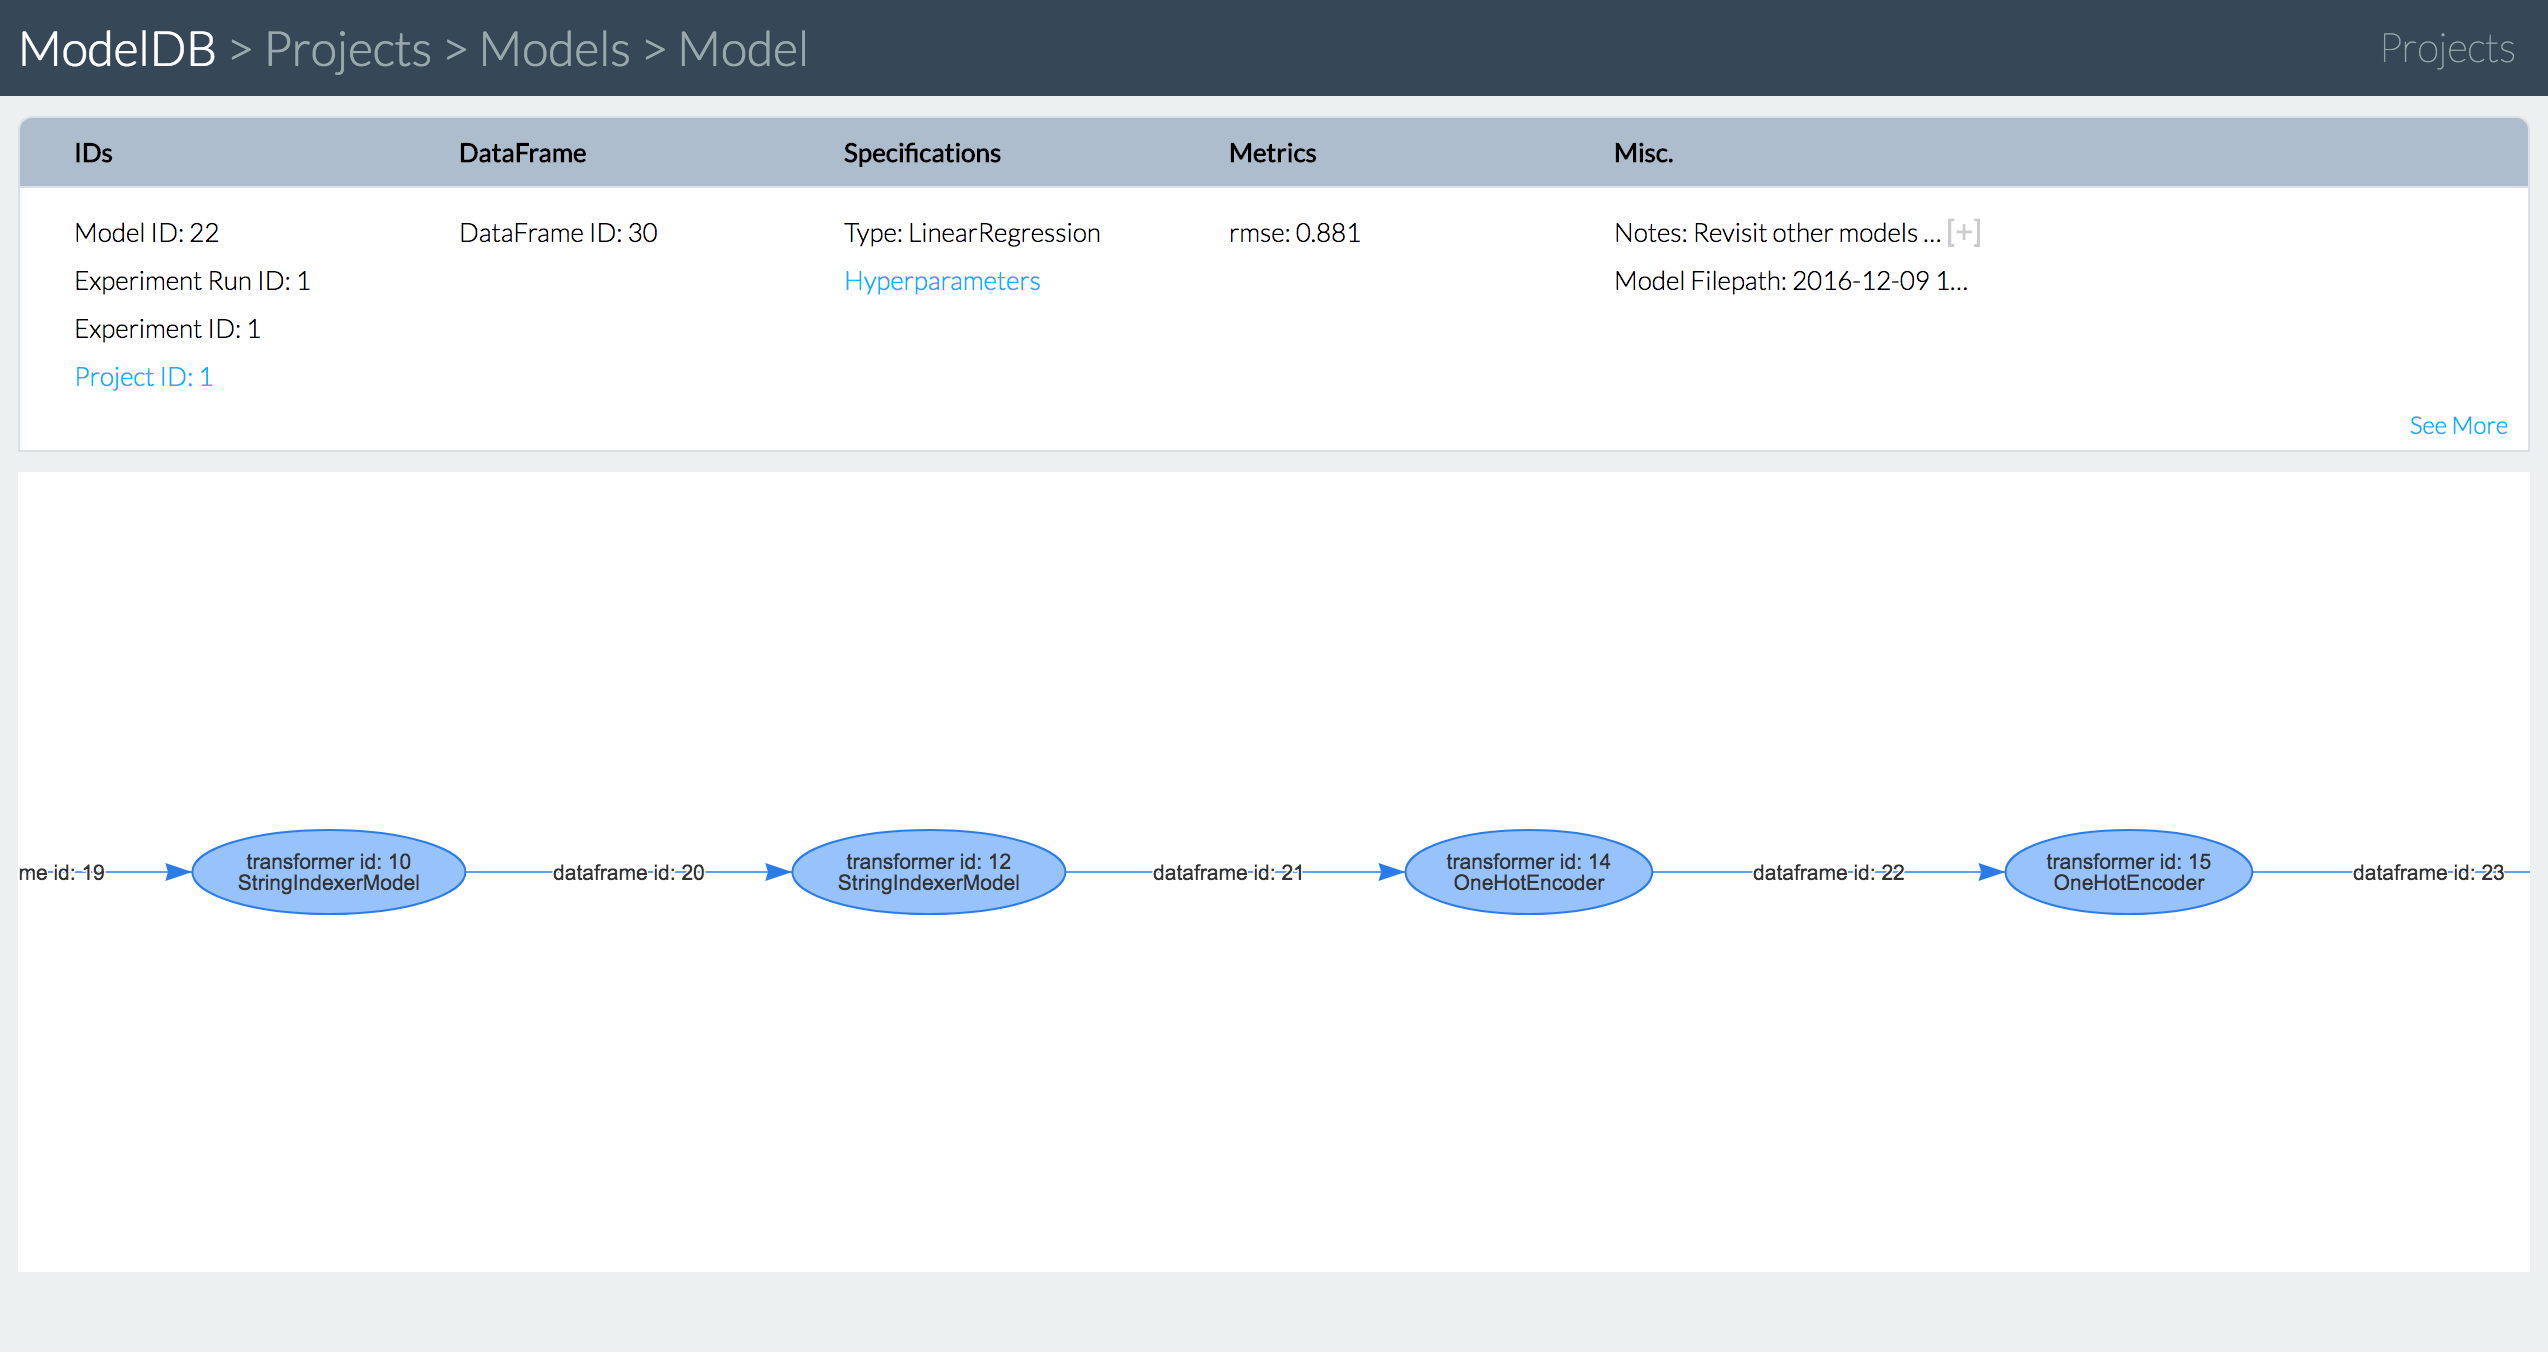
\includegraphics[width=0.48\textwidth]{figs/mdb_model_pipeline.png}
% \end{subfigure}%
% \caption{\zillow pipelines}
% \label{fig:storage_sizes_trad}
% \end{figure*}

\begin{figure*}
  \centering
  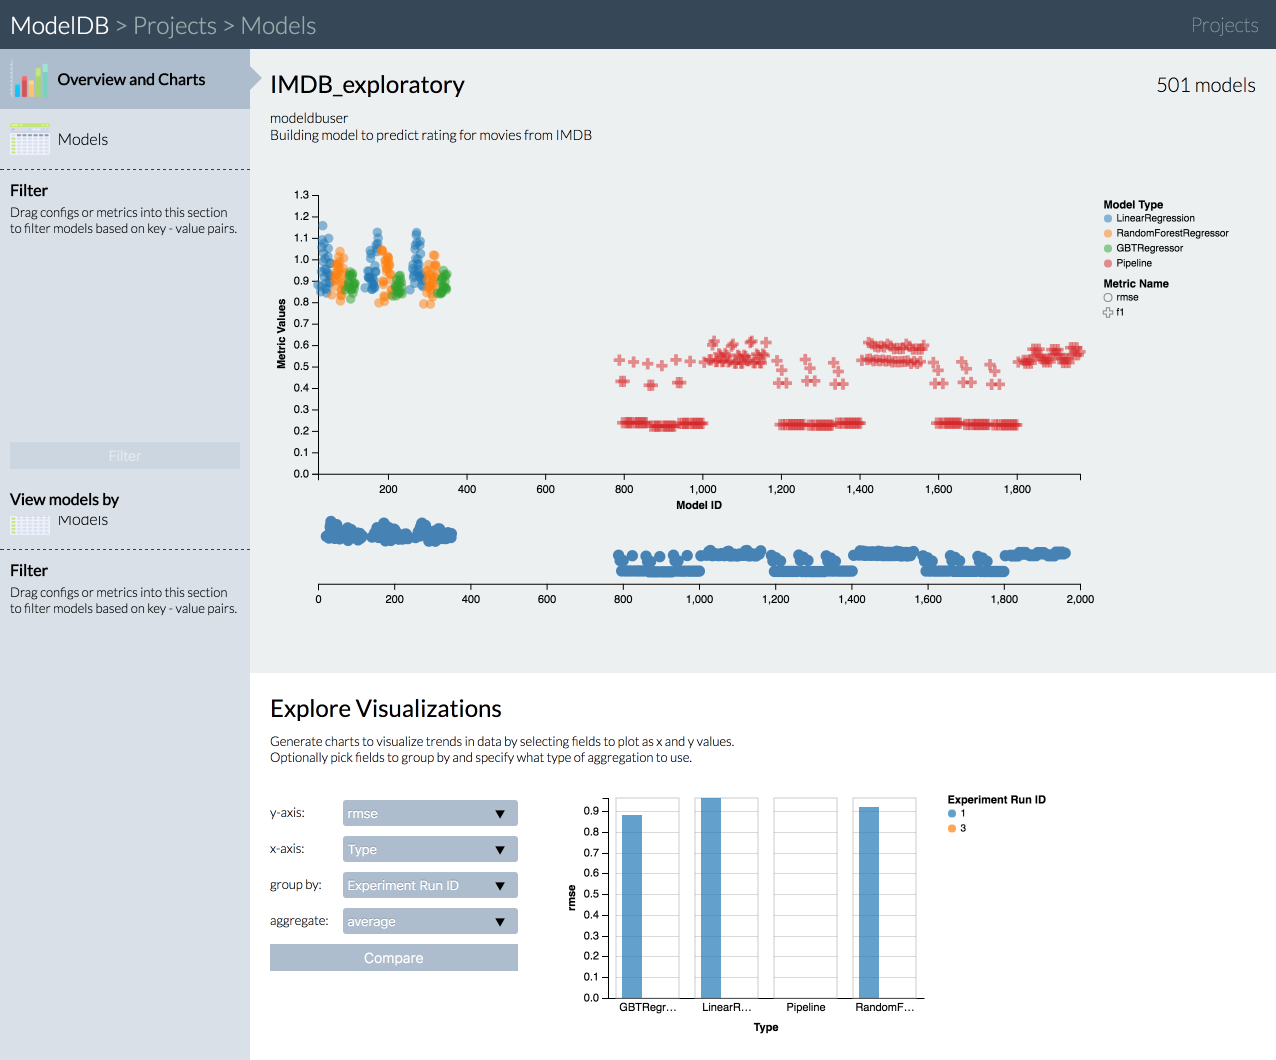
\includegraphics[trim=0mm 0mm 0mm 0mm,
  clip=true, width=0.8\textwidth]{mdb_model_timeline.png}
  \caption{\label{fig:mdb_model_timeline} Model Summary Visualization and Custom Visualization Builder}
\end{figure*}

% \begin{figure*}
%   \centering
%   \includegraphics[trim=0mm 0mm 0mm 0mm,
%   clip=true, width=\textwidth]{figures/mdb_model_timeline_drilldown.png}
%   \caption{\label{fig:mdb_model_timeline_drilldown} Model Timeline Drilldown 
%   (reproduced from~\cite{weiwei})}
% \end{figure*}

% \begin{figure*}
%   \centering
%   \includegraphics[trim=0mm 0mm 0mm 0mm,
%   clip=true, width=\textwidth]{figures/mdb_custom_visualizations.png}
%   \caption{\label{fig:mdb_custom_visualizations} Custom Visualizations
%   (reproduced from~\cite{weiwei})}
% \end{figure*}

\begin{figure*}
  \centering
  \includegraphics[trim=0mm 0mm 0mm 0mm,
  clip=true, width=0.8\textwidth]{mdb_tabular.png}
  \caption{\label{fig:tabular-view} Tabular Models View}
\end{figure*}

% \begin{figure*}
%   \centering
%   \includegraphics[trim=0mm 0mm 0mm 0mm,
%   clip=true, width=\textwidth]{figures/mdb_model_filtering.png}
%   \caption{\label{fig:mdb_model_filtering} Model Filtering
%   (reproduced from~\cite{weiwei})}
% \end{figure*}

% \begin{figure*}
%   \centering
%   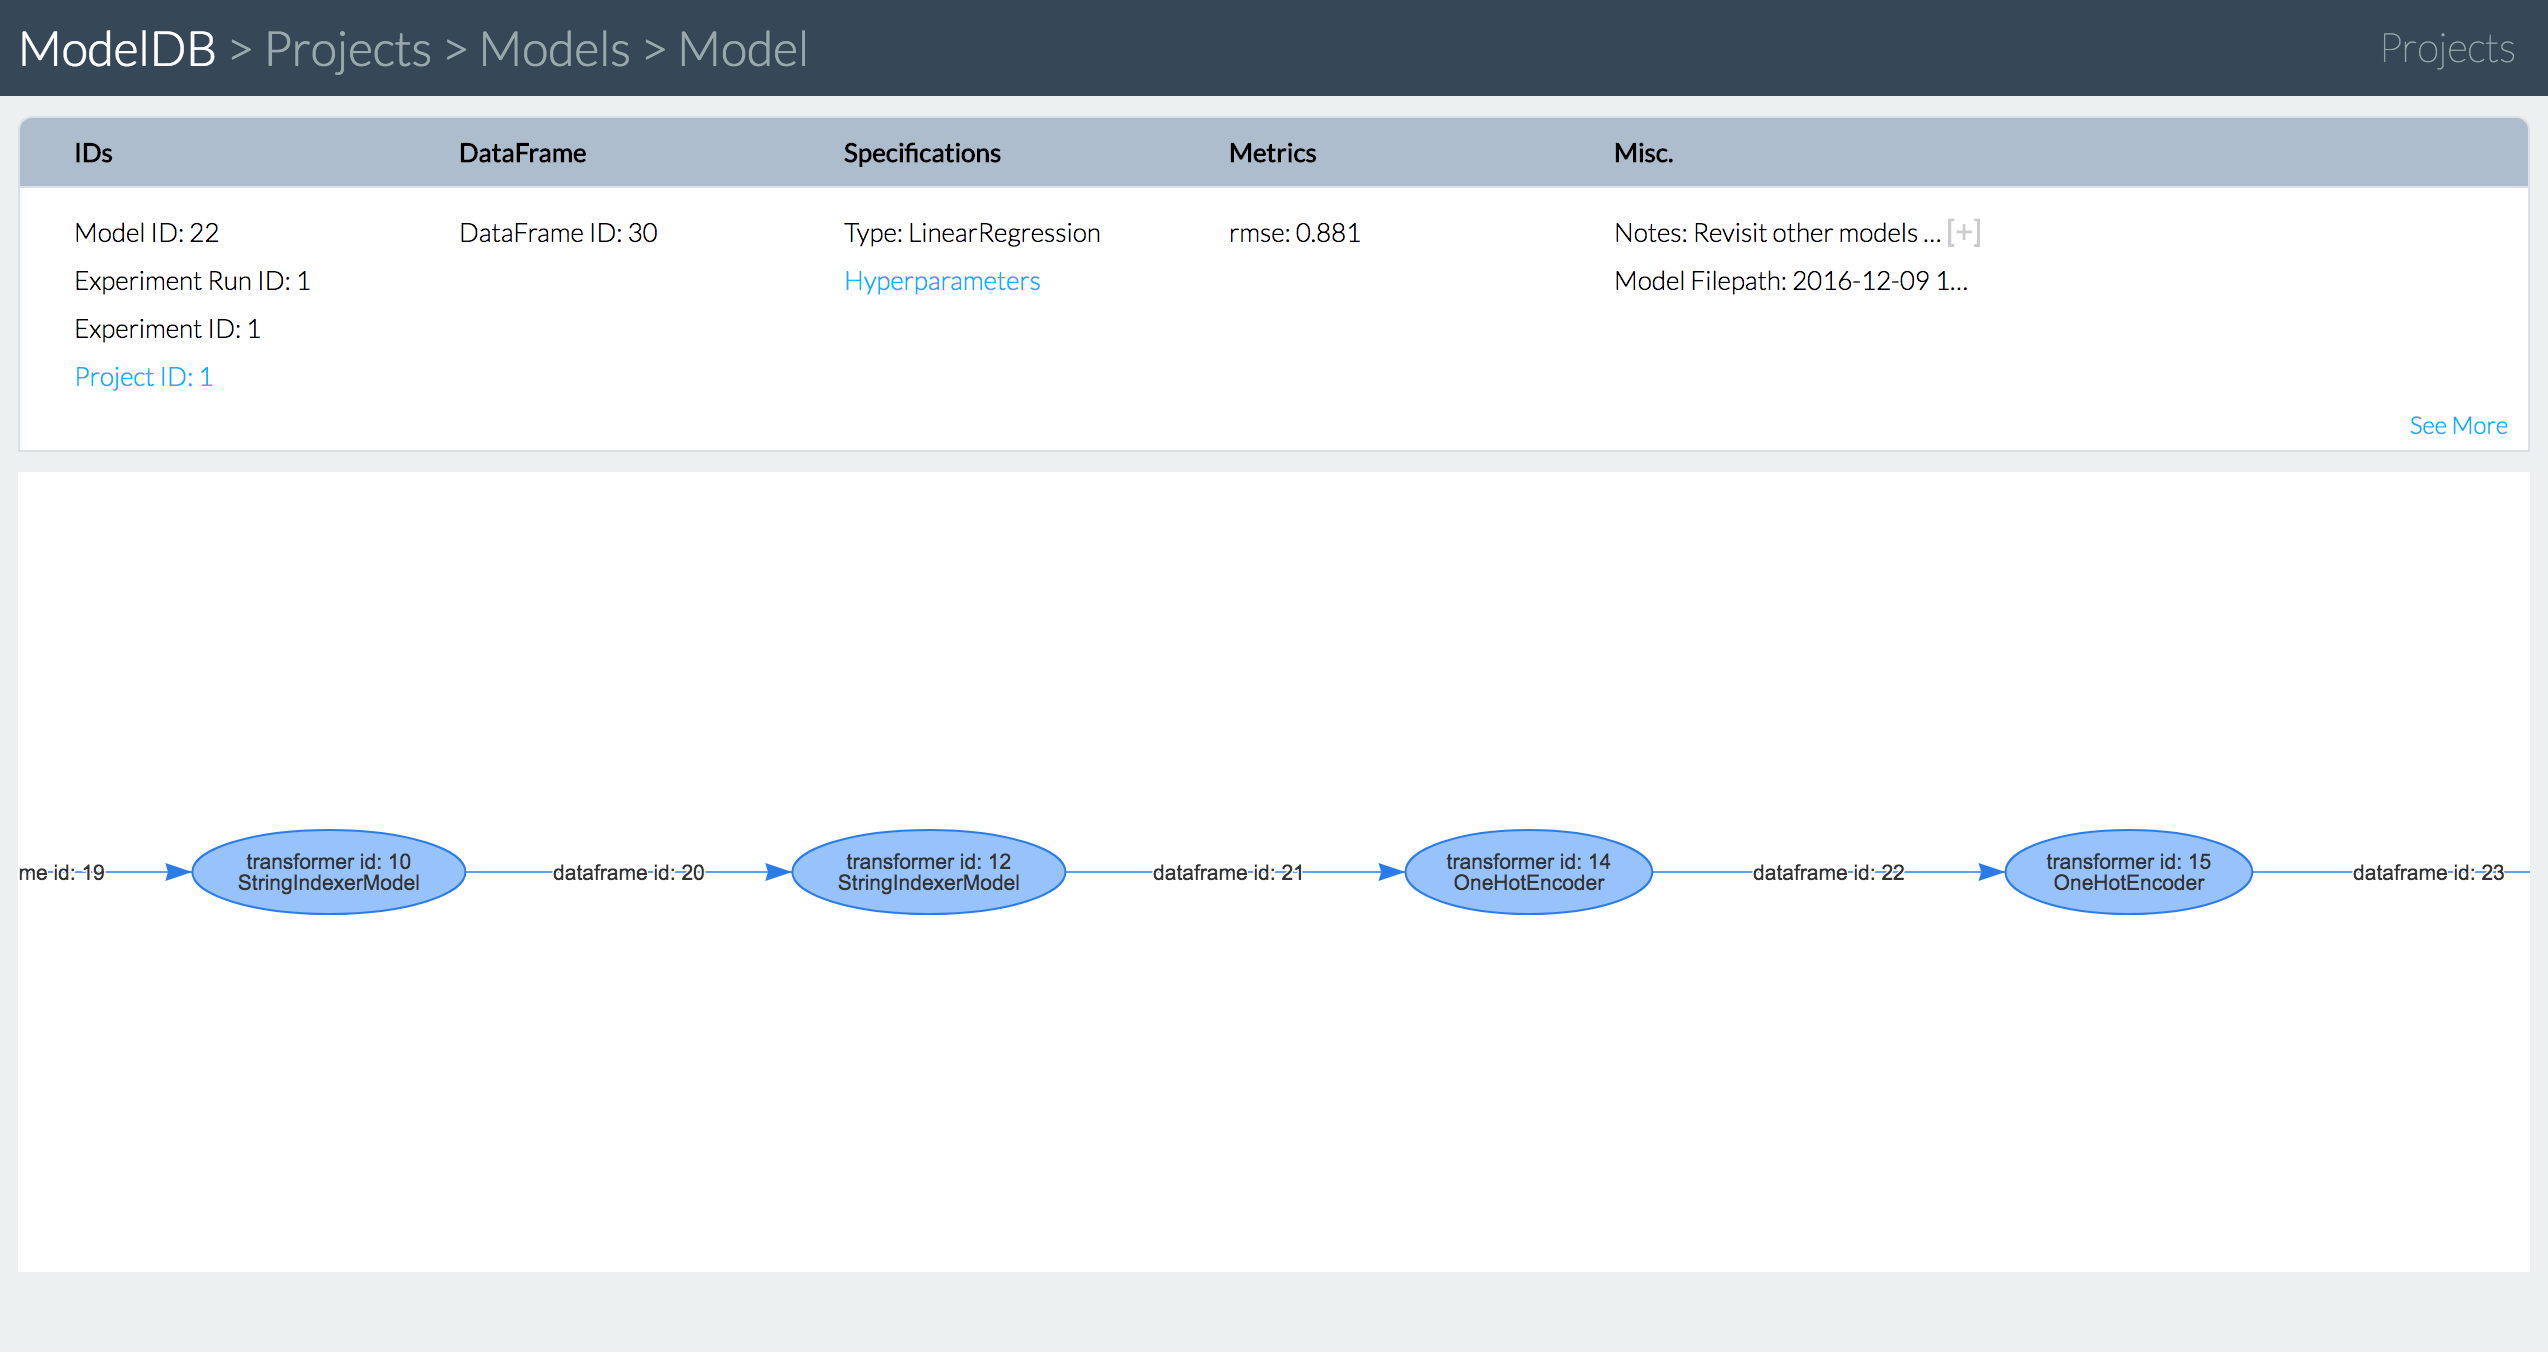
\includegraphics[trim=0mm 0mm 0mm 0mm,
%   clip=true, width=0.75\textwidth]{figs/mdb_model_pipeline.png}
%   \caption{\label{fig:mdb_model_pipeline} Model Pipeline View}
% \end{figure*}
\subsection{\mdb Adoption and Future Work}

We officially released \mdb as an open-source model management system in 
Feb. 2017 and since then there has been a large amount of interest and adoption of \mdb.
Over the last year, our GitHub repository~\cite{mdb-repo} 
has garnered $>$ 500 stars, has been cloned over a thousand times, and has been
forked $>$100 times.
\mdb has been tested at multiple small and large companies and has been deployed in financial institutions.
\mdb has also served as inspiration for other model management systems such as~\cite{mlflow}.
The rapid adoption of \mdb indicates a strong need for model management, and our current work focuses on expanding \mdb to support other phases of the ML life-cycle.
\section{Evolution of Model Management Systems}
\label{sec:future}

As machine learning models proliferate into every business process and product, we posit that the task of managing the life-cycle of models will become as key as managing the life-cycle of code.
Just as version control systems such as SVN and Git made source code development and collaboration robust and rapid, we envision that model management systems will serve a similar purpose in the future.
We imagine model management systems to become the system of record for all models and model-related information.
Current model management systems have focused on tracking models in a limited fashion; consequently, to support diverse ML applications, we expect model management systems to evolve in the following directions.

{\bf Model Data Pipelines.} For many machine learning applications, the ultimate performance of the machine learning model depends on the features or data attributes used by the model.
As a result, when a model is to be reproduced, it requires accurate records of the data and transformations used to produce features.
We expect model management systems to evolve to accurately record data versions (train and test) as well data transformations that are used to generate features.
This metadata may come from a separate data processing or workflow system as opposed to being generated by the model management system, however, the model management system would track all the metadata required to create the model end-to-end.

{\bf Model Interoperability.} One of the key challenges in model management described before is the diversity in ML models and frameworks.
While some frameworks support rapid development, others might be more suitable for deployment in production settings.
Given the rapid proliferation of ML frameworks, we expect model management systems to support, if not provide, a level of interoperability between different ML environments and frameworks (e.g., PMML~\cite{pmml} and ONNX~\cite{onnx} provide a good start).
This will enable \dss to pick and choose the best framework for each phase of the model life-cycle without being tied to a single framework.

{\bf Model Testing.} As more decisions and business logic get delegated to machine learning models, the importance of testing models (similar to code testing) will increase and will become a key part of managing the model life-cycle.
For instance, defining unit tests for models and their input data will become commonplace.
Similarly, we expect integration tests with models to become more prevalent as predictions from one model get used as input for other models.
Finally, we note that as adversarial attacks on models increase, testing of models and edge cases will become key, requiring the development of new techniques to prevent adversarial attacks (e.g., ~\cite{adversarialICLR2015,feinman2017detectAdversarial}). 

{\bf Model Monitoring.} While model testing takes place before a model is deployed, model monitoring takes place once the model is deployed in a live system.
Model monitoring today is largely limited to monitoring system-level metrics such as the number of prediction requests, latency, and compute usage.
However, we are already seeing the need for data-level monitoring of models (e.g., as noted in~\cite{sculley2014high-interest-cc}) to ensure that the offline and live data fed to a model is similar.
We expect model management systems to encompass model monitoring modules to ensure continued model health, triggering alerts and actions as appropriate.

{\bf Model Interpretability and Fairness.} 
As models are used for automated decision making in regulated industries and increasingly used by non-technical users, explaining the results of models will become a key aspect of the management of deployed models (as evidenced by the rich research on interpretability~\cite{shap,DoshiKim2017Interpretability,svcca}).
We view a model management system as the system of record for all models and, therefore, the logical gateway for model interpretability and understanding.
In the future, we therefore expect model management systems to expose interpretability functionality for every recorded model.
\section{Conclusion}
\label{sec:conclusion}
ML models are becoming ubiquitous is a variety of domains.
This proliferation of ML brings to the forefront the need for systems that are responsible for managing models across their entire life-cycle starting with data preparation to model retirement.
In this paper, we discussed the motivation for model management systems as well as challenges associated with consistently tracking models throughout their life-cycle.
We described \mdb, the first open-source model management system developed at MIT.
Finally, we described the evolving opportunities in model management.

\begin{thebibliography}{10} 
\itemsep=1pt 
\begin{small}
\bibitem{bavoil2005vistrails}
Louis Bavoil, Steven~P Callahan, Patricia~J Crossno, Juliana Freire, Carlos~E
  Scheidegger, Cl{\'a}udio~T Silva, and Huy~T Vo.
\newblock Vistrails: Enabling interactive multiple-view visualizations.
\newblock In {\em Visualization, 2005. VIS 05. IEEE}, pages 135--142. IEEE,
  2005.

\bibitem{callahan2006workflows}
Steven~P Callahan, Juliana Freire, Emanuele Santos, Carlos~E Scheidegger,
  Claudio~T Silva, and Huy~T Vo.
\newblock Managing the evolution of dataflows with vistrails.
\newblock In {\em Data Engineering Workshops, 2006. Proceedings. 22nd
  International Conference on}, pages 71--71. IEEE, 2006.

\bibitem{callahan2006vistrails}
Steven~P Callahan, Juliana Freire, Emanuele Santos, Carlos~E Scheidegger,
  Cl{\'a}udio~T Silva, and Huy~T Vo.
\newblock Vistrails: visualization meets data management.
\newblock In {\em Proceedings of the 2006 ACM SIGMOD international conference
  on Management of data}, pages 745--747. ACM, 2006.

\bibitem{toxic-comments}
Kaggle competition.
\newblock Toxic comment classification challenge.
\newblock
  \url{https://www.kaggle.com/c/jigsaw-toxic-comment-classification-challenge}.

\bibitem{zillow}
Kaggle Competition.
\newblock Zillow prize: Zillow’s home value prediction (zestimate).
\newblock \url{https://www.kaggle.com/c/zillow-prize-1}.

\bibitem{DoshiKim2017Interpretability}
Been Doshi-Velez, Finale;~Kim.
\newblock Towards a rigorous science of interpretable machine learning.
\newblock In {\em eprint arXiv:1702.08608}, 2017.

\bibitem{fblearner}
Facebook Engineering.
\newblock Introducing fblearner flow: Facebook's ai backbone.
\newblock
  \url{https://code.facebook.com/posts/1072626246134461/introducing-fblearner-flow-facebook-s-ai-backbone/}.

\bibitem{michelangelo}
Uber Engineering.
\newblock Meet michelangelo: Uber's machine learning platform.
\newblock \url{https://eng.uber.com/michelangelo/}.

\bibitem{feinman2017detectAdversarial}
Reuben Feinman, Ryan~R Curtin, Saurabh Shintre, and Andrew~B Gardner.
\newblock Detecting adversarial samples from artifacts.
\newblock {\em arXiv preprint}, 2017.

\bibitem{adversarialICLR2015}
Ian~J. Goodfellow, Jonathon Shlens, and Christian Szegedy.
\newblock Explaining and harnessing adversarial examples.
\newblock {\em ICLR}, 2015.

\bibitem{airflow}
Apache~Software Foundation.
\newblock Airflow.

\bibitem{mdb-repo}
MIT~DB Group.
\newblock Modeldb.
\newblock \url{https://github.com/mitdbg/modeldb}, 2017.

\bibitem{pmml}
Alex Guazzelli, Wen-Ching Lin, and Tridivesh Jena.
\newblock {\em PMML in Action: Unleashing the Power of Open Standards for Data
  Mining and Predictive Analytics}.
\newblock CreateSpace, Paramount, CA, 2010.

\bibitem{hellerstein2017ground}
Joseph~M Hellerstein, Vikram Sreekanti, Joseph~E Gonzalez, James Dalton, Akon
  Dey, Sreyashi Nag, Krishna Ramachandran, Sudhanshu Arora, Arka Bhattacharyya,
  Shirshanka Das, et~al.
\newblock Ground: A data context service.

\bibitem{msms}
Arun Kumar, Robert McCann, Jeffrey Naughton, and Jignesh~M. Patel.
\newblock Model selection management systems: The next frontier of advanced
  analytics.
\newblock {\em SIGMOD Rec.}, 44(4):17--22, May 2016.

\bibitem{kepler}
Bertram Lud{\"a}scher, Ilkay Altintas, Chad Berkley, Dan Higgins, Efrat Jaeger,
  Matthew Jones, Edward~A Lee, Jing Tao, and Yang Zhao.
\newblock Scientific workflow management and the kepler system.
\newblock {\em Concurrency and Computation: Practice and Experience},
  18(10):1039--1065, 2006.

\bibitem{shap}
Scott~M Lundberg and Su-In Lee.
\newblock A unified approach to interpreting model predictions.
\newblock In {\em Advances in Neural Information Processing Systems 30}, pages
  4768--4777. Curran Associates, Inc., 2017.

\bibitem{modelhub}
H.~Miao, A.~Li, L.~S. Davis, and A.~Deshpande.
\newblock Modelhub: Deep learning lifecycle management.
\newblock In {\em 2017 IEEE 33rd International Conference on Data Engineering
  (ICDE)}, pages 1393--1394, April 2017.

\bibitem{provdb}
Hui Miao, Amit Chavan, and Amol Deshpande.
\newblock Provdb: Lifecycle management of collaborative analysis workflows.
\newblock 2017.

\bibitem{mlflow}
MLFlow.
\newblock Mlflow.
\newblock \url{https://github.com/mlflow/mlflow}.

\bibitem{gdpr}
Official~Journal of~the European~Union.
\newblock General data protection regulation.
\newblock
  \url{https://eur-lex.europa.eu/legal-content/EN/TXT/?uri=celex%3A32016R0679}.

\bibitem{onnx}
ONNX.
\newblock Onnx: Open neural network exchange.
\newblock \url{https://github.com/onnx/onnx}.

\bibitem{svcca}
Maithra Raghu, Justin Gilmer, Jason Yosinski, and Jascha Sohl-Dickstein.
\newblock Svcca: Singular vector canonical correlation analysis for deep
  learning dynamics and interpretability.
\newblock In I.~Guyon, U.~V. Luxburg, S.~Bengio, H.~Wallach, R.~Fergus,
  S.~Vishwanathan, and R.~Garnett, editors, {\em Advances in Neural Information
  Processing Systems 30}, pages 6078--6087. Curran Associates, Inc., 2017.

\bibitem{sas-model-manager}
SAS.
\newblock Sas model manager.
\newblock \url{https://www.sas.com/en_us/software/model-manager.html}.

\bibitem{sculley2014high-interest-cc}
D~Sculley, Todd Phillips, Dietmar Ebner, Vinay Chaudhary, and Michael Young.
\newblock Machine learning: The high-interest credit card of technical debt.

\bibitem{luigi}
Spotify.
\newblock Luigi.
\newblock \url{https://github.com/spotify/luigi}.

\bibitem{galaxy}
The~Galaxy Team and Community.
\newblock The galaxy project.
\newblock \url{https://galaxyproject.org/}.

\bibitem{modeldb-hilda}
Manasi Vartak, Harihar Subramanyam, Wei-En Lee, Srinidhi Viswanathan, Saadiyah
  Husnoo, Samuel Madden, and Matei Zaharia.
\newblock Modeldb: A system for machine learning model management.
\newblock In {\em Proceedings of the Workshop on Human-In-the-Loop Data
  Analytics}, HILDA '16, pages 14:1--14:3, New York, NY, USA, 2016. ACM.

\bibitem{taverna}
Katherine Wolstencroft, Robert Haines, Donal Fellows, Alan Williams, David
  Withers, Stuart Owen, Stian Soiland-Reyes, Ian Dunlop, Aleksandra Nenadic,
  Paul Fisher, et~al.
\newblock The taverna workflow suite: designing and executing workflows of web
  services on the desktop, web or in the cloud.
\newblock {\em Nucleic acids research}, 41(W1):W557--W561, 2013.


\end{small}
\end{thebibliography}
\end{document}